\documentclass[a4paper, 10pt]{article}

\usepackage{graphicx}
\usepackage[T1]{fontenc}
\usepackage[polish]{babel}
\usepackage[utf8]{inputenc}
\usepackage[left=25mm, right=25mm, top=25mm, bottom=25mm]{geometry}
\usepackage{listings}
\usepackage{hyperref}
\usepackage{caption}
\usepackage{float}
\usepackage{xcolor}
\usepackage{color}



\graphicspath{{./figures}}

\renewcommand\contentsname{Spis treści}
\renewcommand\listfigurename{Spis rysunków}
\renewcommand\lstlistingname{Polecenie}
\renewcommand\lstlistlistingname{Spis poleceń}

\definecolor{codegreen}{rgb}{0,0.6,0}
\definecolor{codegray}{rgb}{0.5,0.5,0.5}
\definecolor{codepurple}{HTML}{C42043}
\definecolor{backcolour}{HTML}{F2F2F2}
\definecolor{bookColor}{cmyk}{0,0,0,0.90}

\captionsetup[lstlisting]{
    labelsep=period,
    justification=centering,
    singlelinecheck=false,
    width=0.9\linewidth
}

\captionsetup[figure]{
    justification=centering,
    singlelinecheck=false,
    width=.9\linewidth
}

\lstdefinestyle{SQL}{
    language=SQL,
    backgroundcolor=\color{backcolour},
    basicstyle=\footnotesize\ttfamily,
    breaklines=true,
    captionpos=b,
    commentstyle=\color{green},
    keywordstyle=\color{red},
    stringstyle=\color{red},
    showstringspaces=false,
    tabsize=2,
    morekeywords={USE, CREATE, TABLE, VARCHAR, INT, NOT, NULL, PRIMARY, KEY, AUTO_INCREMENT, INSERT, INTO, VALUES, SELECT, FROM, WHERE, ORDER, BY, ASC, DESC, GROUP, HAVING, UPDATE, SET, DELETE, JOIN, LEFT, RIGHT, OUTER, INNER, ON},
    frame=single,
    framesep=5pt,
    rulecolor=\color{gray},
    linewidth=1\linewidth
}

\begin{document}
\begin{titlepage}
\begin{center}
	
\includegraphics[scale=0.7]{logo.png}

	\vspace*{4cm}
	\textbf{Bazy danych\\ Laboratorium}

	\vspace{1.5cm}
	\textit{Zaawansowane zapytania Oracle}

	\vspace{1.5cm}
	\textbf{Stanislau Antanovich}\\
	nr. indeksu: 173590\\
	gr. lab: L04

	\vspace{4.5cm}
	\today
\end{center}
\end{titlepage}

\tableofcontents
\listoffigures
\lstlistoflistings

\newpage

\section{Wprowadzenie}
\subsection{Cel ćwiczenia}

Cel tego zajęcia polega na rozwinięciu umiejętności praktycznego stosowania róźnorodnych funkcji języka SQL w kontekście pracy z bazą danych. 
Ćwiczenie ma na celu umożliwienie zrozumienia skomplikowanych technik manipulacji danymi.
\subsection{Prygotowanie}

\section{Realizacja}

Po zaimportowaniu bazy danych ``Firma handlowa'' do narzędzia SQL developer można zaczynać  wykonywać polecenia SQL.

\begin{enumerate}

\item Wyświetl id, imię, nazwisko oraz sumę pensji i prowizji każdego z pracowników. Nagłówek kolumny wynikowej z sumą pensji i prowizji nazwij `Wartość' (AS). 

\begin{lstlisting}[style=SQL, caption=\textit{Wyświetlenie id, imia, nazwiska oraz sumy pensji i prowizji każdego z pracowników}]
SELECT ID_PRACOWNIKA,IMIE,NAZWISKO,(PENSJA+PROWIZJA) AS Wartosc FROM PRACOWNICY;
\end{lstlisting}

\begin{figure}[H]
	\centering
	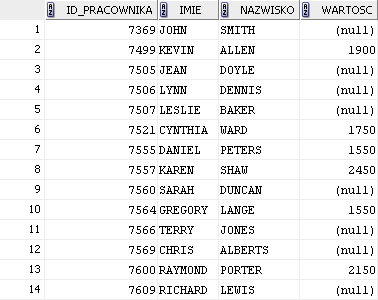
\includegraphics[scale=0.7]{zadanie1.png}
	\caption{\textit{Wyświetlenie id, imia, nazwiska, oraz sumy pensji i prowizji każdego z pracowników}}
\end{figure}

\item Wyświetlenie danych pracowników po 0.1\% podwyżce.
\begin{lstlisting}[style=SQL, caption=\textit{Wyświetlenie danych pracowników po 0.1 podwyżce}]
SELECT ID_PRACOWNIKA, IMIE, NAZWISKO, PENSJA * 1.001 AS PENSJA FROM PRACOWNICY;
\end{lstlisting}

\begin{figure}[H]
	\centering
	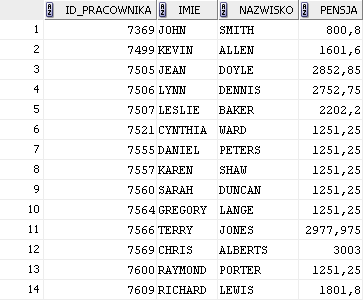
\includegraphics[scale=0.7]{zadanie2.png}
	\caption{\textit{Wyświetlenie danych pracowników po 0.1 podwyżce}}
\end{figure}


\item Wyświetlenie wszystkich pracowników z nieznaną prowizji.  
\begin{lstlisting}[style=SQL, caption=\textit{Wyświetlenie wszystkich pracowników z nieznaną prowizji}]
SELECT * FROM PRACOWNICY WHERE PROWIZJA IS NULL;
\end{lstlisting}

\begin{figure}[H]
	\centering
	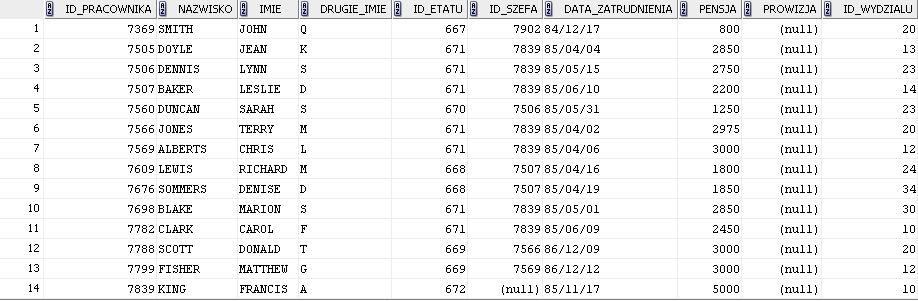
\includegraphics[scale=0.7]{zadanie3.png}
	\caption{\textit{Wyświetlenie wszystkich pracowników z nieznaną prowizji}}
\end{figure}


\item Wyświetlenie danych wszystkich klientów niepochodzących z miasta `BURLINGAME'. Wykorzystaj operator IN. 
\begin{lstlisting}[style=SQL, caption=\textit{Wyświetlenie danych wszystkich klientów niepochodzących z miasta `BURLINGANE'}]
SELECT * FROM KLIENCI WHERE MIASTO NOT IN ('BURLINGAME');
\end{lstlisting}

\begin{figure}[H]
	\centering
	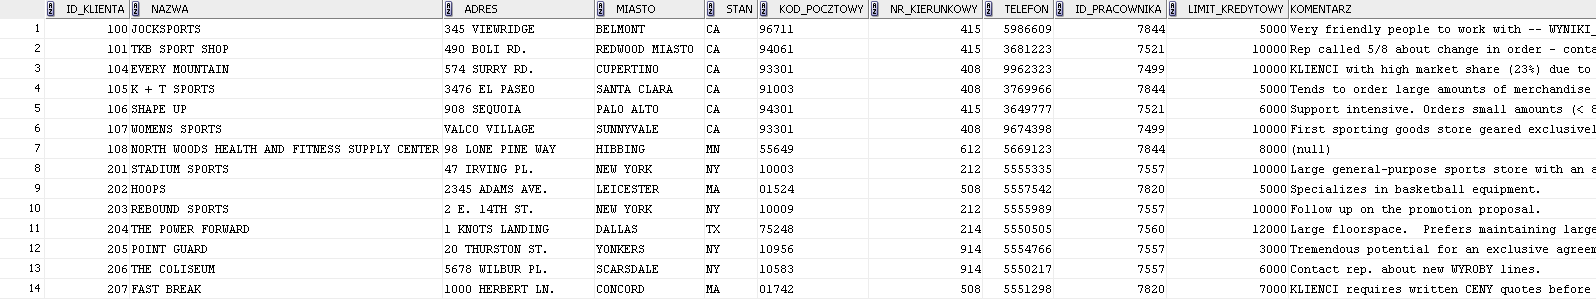
\includegraphics[scale=0.5]{zadanie4.png}
	\caption{\textit{Wyświetlenie danych wszystkich klientów niepochodzących z miasta `BURLINGAME'}}
\end{figure}


\item Wyświetlenie imion i nazwisk pracowników z prowizją o wartości w przedziale: <500;900>. Wykorzystaj operator BETWEEN. 
\begin{lstlisting}[style=SQL, caption=\textit{Wyświetlenie imion i nazwisk pracowników z prowizją o wartości w przedziale: <500;900>}]
SELECT IMIE, NAZWISKO FROM PRACOWNICY WHERE PROWIZJA BETWEEN 500 AND 900;
\end{lstlisting}

\begin{figure}[H]
	\centering
	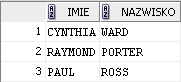
\includegraphics[scale=0.7]{zadanie5.png}
	\caption{\textit{Wyświetlenie imion i nazwisk pracowników z prowizją o wartości w przedziale: <500;900>}}
\end{figure}


\item Zlicz ilość rekordów w tabeli `KLIENCI'. 
\begin{lstlisting}[style=SQL]
\end{lstlisting}


\item  Zwróć wartość najwyższej pensji, jaką ma pracownik w tabeli `PRACOWNICY'.  
\begin{lstlisting}[style=SQL]
\end{lstlisting}


\item Zwróć średnią arytmetyczną wszystkich pensji pracowników z etatu `MANAGER'.  
\begin{lstlisting}[style=SQL]
\end{lstlisting}


\item Wyświetl wszystkich pracowników wraz z wydziałami, do których należą.
\begin{lstlisting}[style=SQL]
\end{lstlisting}


\item Wykonaj poprzednie zadanie z użyciem SQL Alias. Rezultat posortuj na podstawie wydziału i nazwiska pracownika.  
\begin{lstlisting}[style=SQL]
\end{lstlisting}


\item Pobierz pracowników o etacie z literą `L' w nazwie. Wykorzystaj INNER JOIN do połączenia tabel. 
\begin{lstlisting}[style=SQL]
\end{lstlisting}


\item Pobierz pracowników o etacie z literą `L' w nazwie. Wykorzystaj WHERE do połączenia tabel. 
\begin{lstlisting}[style=SQL]
\end{lstlisting}


\item Wyświetl wszystkich pracowników, którzy związani są z siedzibami ``NEW YORK'' i ``DALLAS''. 
\begin{lstlisting}[style=SQL]
\end{lstlisting}


\item Zlicz ilość wszystkich pracowników poszczególnych etatów. Wykorzystaj grupowanie. 
\begin{lstlisting}[style=SQL]
\end{lstlisting}


\item Podaj sumę wszystkich pensji z poszczególnych etatów (etat;suma).
\begin{lstlisting}[style=SQL]
\end{lstlisting}


\item Zlicz ilość wszystkich pracowników poszczególnych wydziałów, których liczebność jest większa niż 4.  
\begin{lstlisting}[style=SQL]
\end{lstlisting}


\item Wyświetl najmniej liczny wydział w firmie (ilość pracowników).
\begin{lstlisting}[style=SQL]
\end{lstlisting}
\end{enumerate}


\section{Wnioski}

\end{document}
